%%%% Modelo de comportamiento %%%%

\section{Módulos}

	La figura \ref{modulos} muestra los módulos del sistema a desarrollar.

	%Módulos del sistema
	\begin{figure}[h]
		
		\begin{center}

			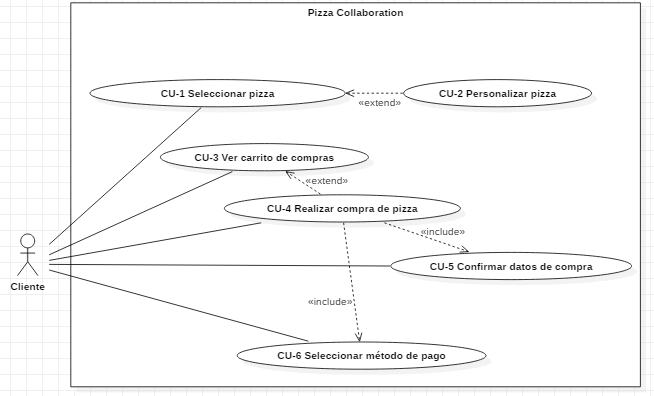
\includegraphics[scale=0.60]{imagenes/modulos/Modulos-PizzaCollaboration.png}
			\caption{Módulos del sistema}
			\label{modulos}
			
		\end{center}
		
	\end{figure}

	A continuación se describe de manera general cada uno de los módulos.

	\begin{itemize}

		\item \textit{A}. Descripción general del módulo A.
		\item \textit{B}. Descripción general del módulo B.
		\item \textit{Registro de solicitantes}. Permite a los solicitantes obtener una cuenta de usuario en el sistema para poder solicitar servicios a la empresa.
		\item \textit{N}. Descripción general del módulo N.

	\end{itemize}


